\chapter{Specifikacija programske potpore}
		
	\section{Funkcionalni zahtjevi}
			
			\textbf{\textit{dio 1. revizije}}\\
			
			\textit{Navesti \textbf{dionike} koji imaju \textbf{interes u ovom sustavu} ili  \textbf{su nositelji odgovornosti}. To su prije svega korisnici, ali i administratori sustava, naručitelji, razvojni tim.}\\
				
			\textit{Navesti \textbf{aktore} koji izravno \textbf{koriste} ili \textbf{komuniciraju sa sustavom}. Oni mogu imati inicijatorsku ulogu, tj. započinju određene procese u sustavu ili samo sudioničku ulogu, tj. obavljaju određeni posao. Za svakog aktora navesti funkcionalne zahtjeve koji se na njega odnose.}\\
			
			
			\noindent \textbf{Dionici:}
			
			\begin{packed_enum}
				
				\item Dionik 1
				\item Dionik 2				
				\item ...
				
			\end{packed_enum}
			
			\noindent \textbf{Aktori i njihovi funkcionalni zahtjevi:}
			
			
			\begin{packed_enum}
				\item  \underbar{Aktor 1 (inicijator) može:}
				
				\begin{packed_enum}
					
					\item funkcionalnost 1
					\item funkcionalnost 2
					\begin{packed_enum}
						
						\item  podfunkcionalnost 1 
						\item  podfunkcionalnost 2
				
					\end{packed_enum}
					\item  funkcionalnost 3
					
				\end{packed_enum}
			
				\item  \underbar{Aktor 2 (sudionik) može:}
				
				\begin{packed_enum}
					
					\item funkcionalnost 1
					\item funkcionalnost 2
					
				\end{packed_enum}
			\end{packed_enum}
			
			\eject 
			
			
				
			\subsection{Obrasci uporabe}
				
				\textbf{\textit{dio 1. revizije}}
				
				\subsubsection{Opis obrazaca uporabe}
					\textit{Funkcionalne zahtjeve razraditi u obliku obrazaca uporabe. Svaki obrazac je potrebno razraditi prema donjem predlošku. Ukoliko u nekom koraku može doći do odstupanja, potrebno je to odstupanje opisati i po mogućnosti ponuditi rješenje kojim bi se tijek obrasca vratio na osnovni tijek.}\\
					
					%ovaj dio cu ostaviti za copy-paste template
					\noindent \underbar{\textbf{UC$<$broj obrasca$>$ -$<$ime obrasca$>$}}
					\begin{packed_item}
	
						\item \textbf{Glavni sudionik: }$<$sudionik$>$
						\item  \textbf{Cilj:} $<$cilj$>$
						\item  \textbf{Sudionici:} $<$sudionici$>$
						\item  \textbf{Preduvjet:} $<$preduvjet$>$
						\item  \textbf{Opis osnovnog tijeka:}
						
						\item[] \begin{packed_enum}
	
							\item $<$opis korak jedan$>$
							\item $<$opis korak dva$>$
							\item $<$opis korak tri$>$
							\item $<$opis korak četiri$>$
							\item $<$opis korak pet$>$
						\end{packed_enum}
						
						\item  \textbf{Opis mogućih odstupanja:}
						
						\item[] \begin{packed_item}
	
							\item[2.a] $<$opis mogućeg scenarija odstupanja u koraku 2$>$
							\item[] \begin{packed_enum}
								
								\item $<$opis rješenja mogućeg scenarija korak 1$>$
								\item $<$opis rješenja mogućeg scenarija korak 2$>$
								
							\end{packed_enum}
							\item[2.b] $<$opis mogućeg scenarija odstupanja u koraku 2$>$
							\item[3.a] $<$opis mogućeg scenarija odstupanja  u koraku 3$>$
							
						\end{packed_item}
					\end{packed_item}
					%kraj template-a
					
					\noindent \underbar{\textbf{UC25 -Slanje prijave za trenera}}
					\begin{packed_item}
	
						\item \textbf{Glavni sudionik: }Klijent
						\item  \textbf{Cilj:} Klijent šalje prijavu određenom klubu kako bi postao njihov trener
						\item  \textbf{Sudionici:} Baza podataka, klub
						\item  \textbf{Opis osnovnog tijeka:						
						}
						
						\item[] \begin{packed_enum}
	
							\item Klijent odabire određeni klub
							\item Klijent odabire opciju slanja prijave za trenera
							\item Otvara se prozor sa formom za unos osobnih podataka i datoteka – motivacijsko pismo i potvrda o sposobnosti vođenja tečaja
							\item Klijent unosi podatke i potvrđuje slanje
							\item Podaci se pohranjuju u bazu podataka
							\item Klubu se aplikaciji prikazuje nova prijava
						\end{packed_enum}
						
						\item  \textbf{Opis mogućih odstupanja:}
						
						\item[] \begin{packed_item}
	
							\item[4.a] Podaci u formi imaju krivi format ili nisu ispunjena obavezna polja
							\item[] \begin{packed_enum}
								
								\item Aplikacija obavještava klijenta da unese ispravne i obavezne podatke
																
							\end{packed_enum}
														
						\end{packed_item}
					\end{packed_item}
					
					
					\noindent \underbar{\textbf{UC26 – Potvrda prijave za trenera}}
					\begin{packed_item}
	
						\item \textbf{Glavni sudionik: }Klub
						\item  \textbf{Cilj:} Klijent postaje trener u određenom klubu
						\item  \textbf{Sudionici:} Baza podataka, klijent
						\item  \textbf{Preduvjet:} Klijent poslao prijavu za trenera
						\item  \textbf{Opis osnovnog tijeka:}
						
						\item[] \begin{packed_enum}
	
							\item Klub odabire prijavu od određenog klijenta
							\item Klub potvrđuje prijavu
							\item Klijentu se dodjeljuju ovlasti trenera
							\item Prijava se označava kao obrađena
						\end{packed_enum}
							
						\end{packed_item}
					\end{packed_item}
					
					\noindent \underbar{\textbf{UC27 - Odbijanje prijave za trenera}}
					\begin{packed_item}
	
						\item \textbf{Glavni sudionik: }Klub
						\item  \textbf{Cilj:} Klijentu se odbija poslana prijava za trenera
						\item  \textbf{Sudionici:} Baza podataka, klijent
						\item  \textbf{Preduvjet:} Klijent poslao prijavu za trenera
						\item  \textbf{Opis osnovnog tijeka:}
						
						\item[] \begin{packed_enum}
	
							\item Klub odabire prijavu od određenog klijenta
$>$
							\item Klub odbija određenog klijentaa
							\item Prijava se označava kao obrađena
						\end{packed_enum}
						\end{packed_item}
					\end{packed_item}
					
					\noindent \underbar{\textbf{UC28 – Pregled vođenih tečajeva}}
					\begin{packed_item}
	
						\item \textbf{Glavni sudionik: }Trener
						\item  \textbf{Cilj:} Vidjeti popis tečajeva koje vodi
						\item  \textbf{Sudionici:} Baza podataka
						\item  \textbf{Preduvjet:} Trener vodi tečaj za određeni klub
						\item  \textbf{Opis osnovnog tijeka:}
						
						\item[] \begin{packed_enum}
	
							\item Trener odabire opciju za prikaz svojih tečajeva
							\item Aplikacije prikazuje popis tečajeva koje trener vodi
							\item Trener odabire određeni tečaj
							\item Prikazuje se naziv tečaja sa opisom i nužnim informacijama o tečaju
						\end{packed_enum}
						
						\end{packed_item}
					\end{packed_item}
				
				
					\noindent \underbar{\textbf{UC29 - Pregled kalendara s vođenim terminima}}
					\begin{packed_item}
	
						\item \textbf{Glavni sudionik: }Trener
						\item  \textbf{Cilj:} Vidjeti kalendar s popisom treninga koje vodi određenog dana i sata
						\item  \textbf{Sudionici:} Baza podataka
						\item  \textbf{Opis osnovnog tijeka:}
						
						\item[] \begin{packed_enum}
	
							\item Trener odabire opciju za prikaz svojih vođenih termina
							\item Prikazuje se kalendar s označenim terminima kada vodi tečaj
						\end{packed_enum}
						\end{packed_item}
					\end{packed_item}
					
					\noindent \underbar{\textbf{UC30 - Pregled polaznika }}
					\begin{packed_item}
	
						\item \textbf{Glavni sudionik: }Trener
						\item  \textbf{Cilj:} Vidjeti popis nazočnih sudionika na tečaju
						\item  \textbf{Sudionici:} Baza podataka
						\item  \textbf{Preduvjet:} Trener vodi odabrani tečaj
						\item  \textbf{Opis osnovnog tijeka:}
						
						\item[] \begin{packed_enum}
	
							\item Trener odabire određeni tečaja iz popisa tečajeva
							\item Prikazuje se popis sudionika na tečaju s osnovnim osobnim podacima
						\end{packed_enum}
						
						\end{packed_item}
					\end{packed_item}
					
				\subsubsection{Dijagrami obrazaca uporabe}
					
					\textit{Prikazati odnos aktora i obrazaca uporabe odgovarajućim UML dijagramom. Nije nužno nacrtati sve na jednom dijagramu. Modelirati po razinama apstrakcije i skupovima srodnih funkcionalnosti.}
				\eject		
				
				\begin{figure}[H]
			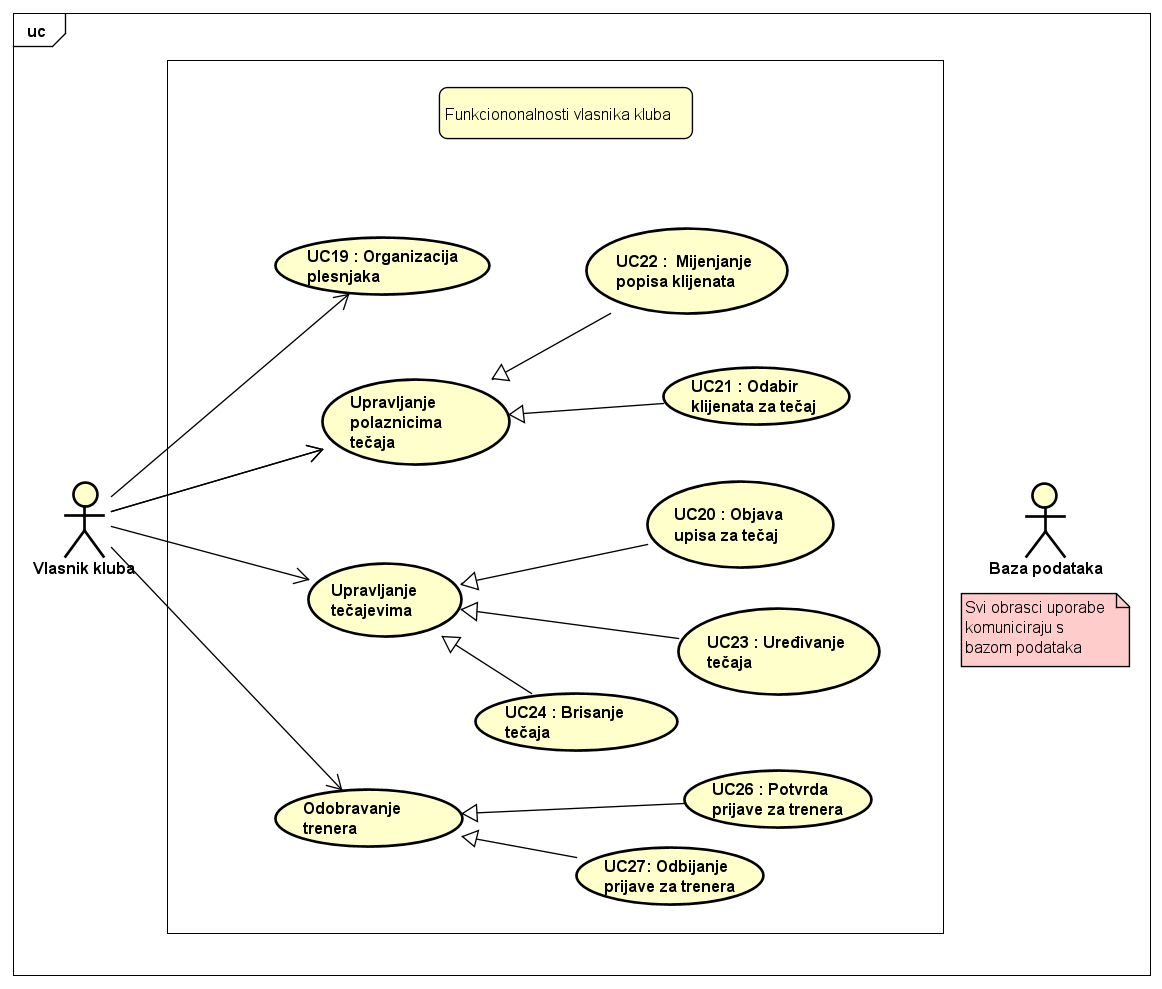
\includegraphics[scale=0.4]{slike/UC_klub.PNG} %veličina u odnosu na širinu linije
			\caption{Dijagram obrasca uporabe, funkcionalnost vlasnika kluba.}
			\label{fig:UC_klub} %label mora biti drugaciji za svaku sliku
		\end{figure}
		
		\begin{figure}[H]
			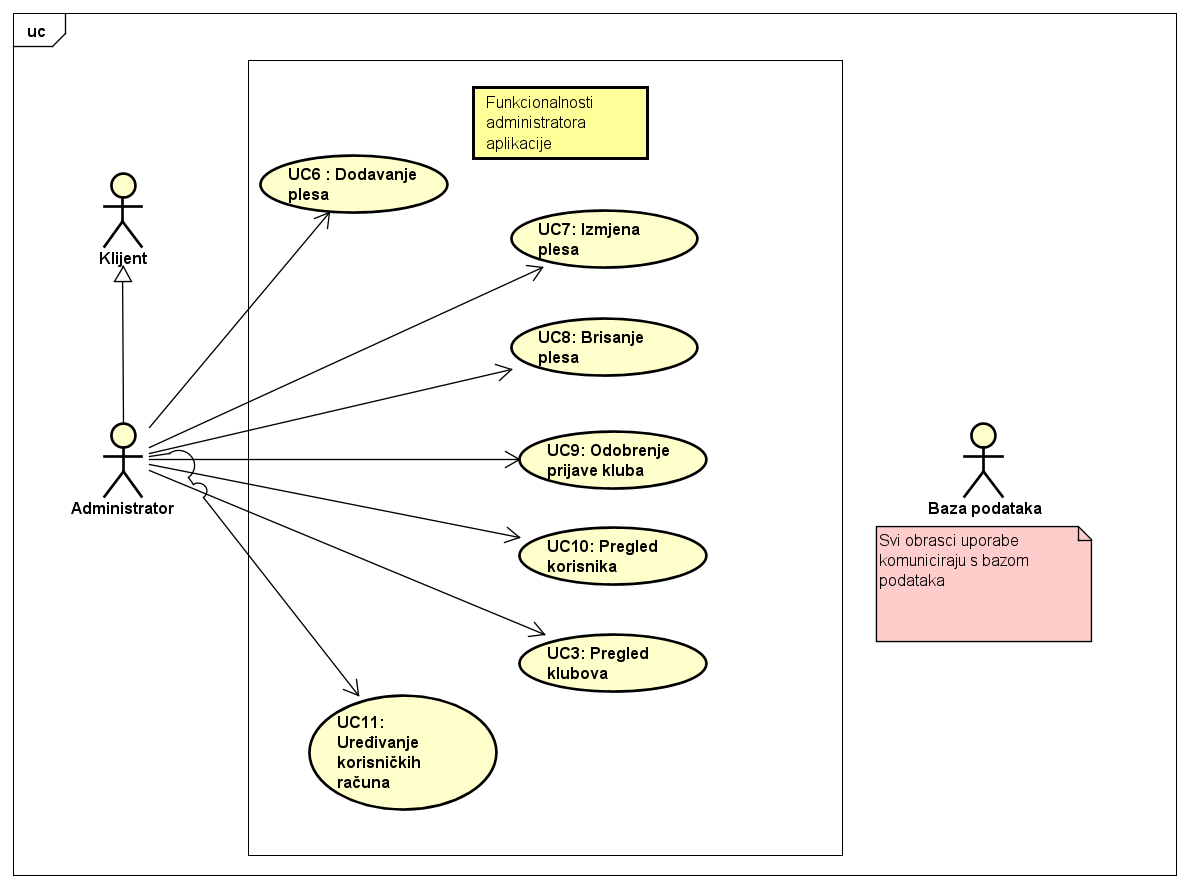
\includegraphics[scale=0.4]{slike/UC_admin.PNG} %veličina u odnosu na širinu linije
			\caption{Dijagram obrasca uporabe, funkcionalnost administratora.}
			\label{fig:UC_admin} %label mora biti drugaciji za svaku sliku
		\end{figure}
		
		
				
			\subsection{Sekvencijski dijagrami}
				
				\textbf{\textit{dio 1. revizije}}\\
				
				\textit{Nacrtati sekvencijske dijagrame koji modeliraju najvažnije dijelove sustava (max. 4 dijagrama). Ukoliko postoji nedoumica oko odabira, razjasniti s asistentom. Uz svaki dijagram napisati detaljni opis dijagrama.}
				\eject
	
		\section{Ostali zahtjevi}
		
			\textbf{\textit{dio 1. revizije}}\\
		 
			 \textit{Nefunkcionalni zahtjevi i zahtjevi domene primjene dopunjuju funkcionalne zahtjeve. Oni opisuju \textbf{kako se sustav treba ponašati} i koja \textbf{ograničenja} treba poštivati (performanse, korisničko iskustvo, pouzdanost, standardi kvalitete, sigurnost...). Primjeri takvih zahtjeva u Vašem projektu mogu biti: podržani jezici korisničkog sučelja, vrijeme odziva, najveći mogući podržani broj korisnika, podržane web/mobilne platforme, razina zaštite (protokoli komunikacije, kriptiranje...)... Svaki takav zahtjev potrebno je navesti u jednoj ili dvije rečenice.}
			 
			 
			 
	